\section{Firmware, Peripherals and Telemetry Contract}
\label{app:firmware}

\subsection{Scheduling}
\begin{table}[htbp]\centering\small
\caption{Execution contexts of the firmware (bare-metal superloop plus interrupts; no RTOS).}
\label{tab:sched}
\begin{tabularx}{\linewidth}{p{3.5cm} p{3.2cm} p{1.6cm} X}
\toprule
Context & Trigger / priority & Rate & Work\\
\midrule
\code{app\_ctrl\_isr} & HRTIM master repetition IRQ, NVIC prio 1 & 10\,kHz ($T_s = 100\us$) & hall averages + OC latch, gain swap, soft-start / \code{stack\_step} / OL duties / pre-bias, slew limit, write CMP1\\
\code{app\_tick\_1ms} & SysTick, prio 0 & 1\,kHz & ms counter; main-loop stall check ($>20\ms$ while switching $\Rightarrow$ fault 0x2000)\\
\code{app\_task\_sense\_v} & main loop & 1\,kHz & INA239 $\times$3 over SPI3 $\rightarrow V_{M1..3}$, die temperatures\\
\code{app\_task\_safety} & main loop, every 10th pass & 100\,Hz & IWDG kick, OV/UV/string-OV, watchdogs, state machine\\
\code{app\_task\_telemetry} & every 20th pass & 50\,Hz & \code{T} frame; \code{S} line at 1\,Hz and on state change\\
\code{app\_task\_cmd} & every pass & 1\,kHz & parse \code{C,...} lines, answer \code{A,...}\\
E-stop & EXTI0 on PC0, prio 0 & event & \code{trip(FLT\_ESTOP)}\\
LPUART1 RX & prio 6, 1 byte per IRQ & event & 512-byte ring buffer\\
\bottomrule
\end{tabularx}
\end{table}
Clock: HSI 16\,MHz $\rightarrow$ PLL $\rightarrow$ SYSCLK 170\,MHz (AHB/APB 170\,MHz, flash latency 4, boost scale); the 400\,kHz build feeds the ADCs from PLL-P at 56.7\,MHz. IWDG 0.3\,s. ISR cost is measured with the DWT cycle counter against the 100\,$\mu$s budget (Release \code{-O2}; \code{-O0} reached 75\,$\mu$s idle and $>100\,\mu$s in CL at 300\,kHz). Toolchain: CMake $\ge$ 3.22, Ninja, arm-none-eabi-gcc (Cortex-M4F, hard float, nano specs), presets Debug/Release; \code{build\_wsl.sh} uses the Windows STM32Cube bundle from WSL.

\subsection{Board routing and current sampling}
\begin{figure}[htbp]
  \centering
  \begin{subfigure}[t]{0.42\linewidth}\centering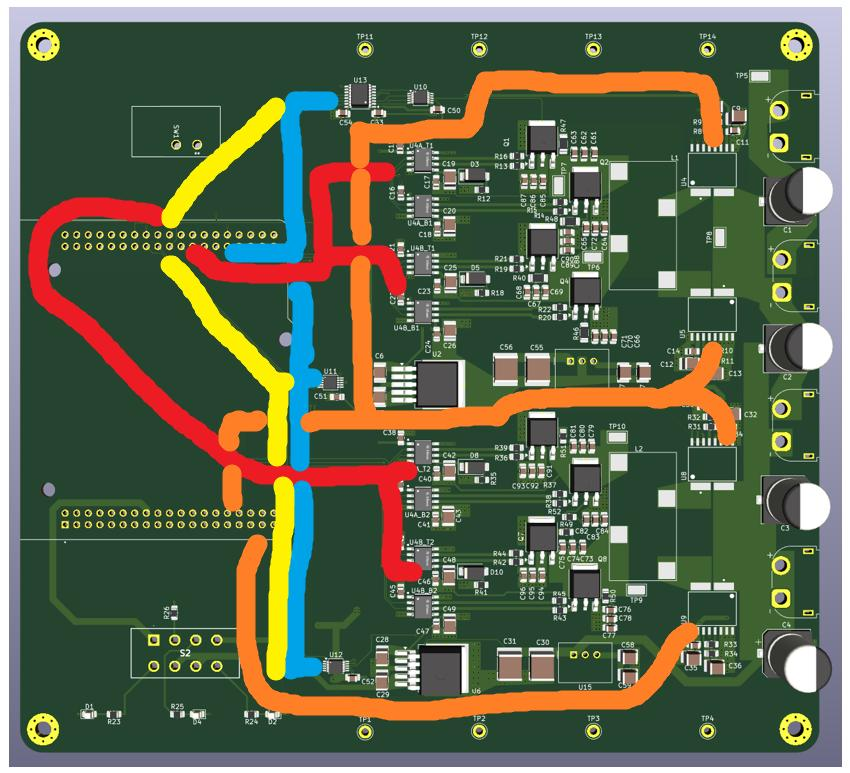
\includegraphics[width=\linewidth]{img-018-026}\caption[{Routing on the Version 0 board}]{Routing on the Version 0 board: PWM (red), SPI (blue), chip selects (yellow), ADC (orange), top and bottom layers.}\end{subfigure}\hfill
  \begin{subfigure}[t]{0.55\linewidth}\centering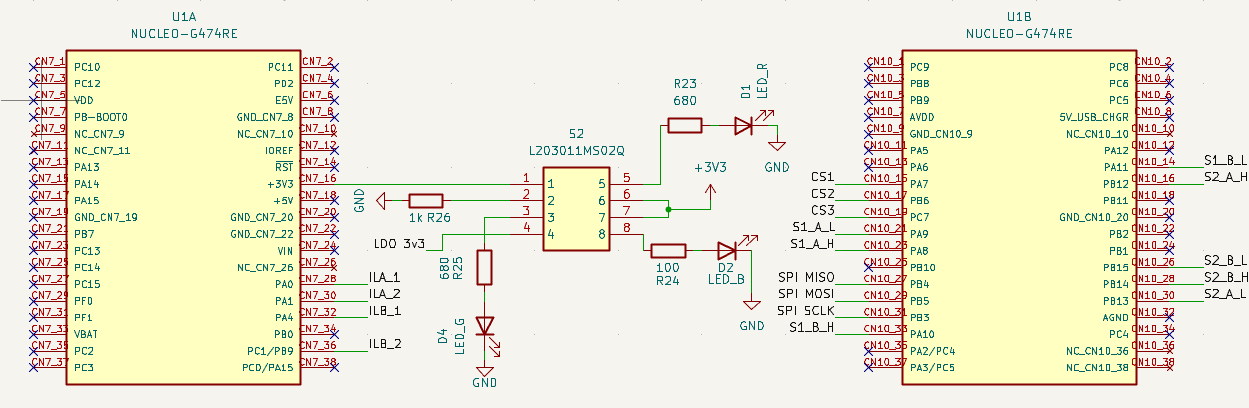
\includegraphics[width=\linewidth]{img-018-028}\caption{Nucleo header pinout used by the PCB.}\end{subfigure}
  \caption{Controller routing on the Version 0 PCB.}
  \label{fig:routing}
\end{figure}
\begin{figure}[htbp]
  \centering
  \resizebox{0.95\linewidth}{!}{% Hall-current sampling: 4 ADC triggers per PWM period from the HRTIM, 80-sample box average per control tick
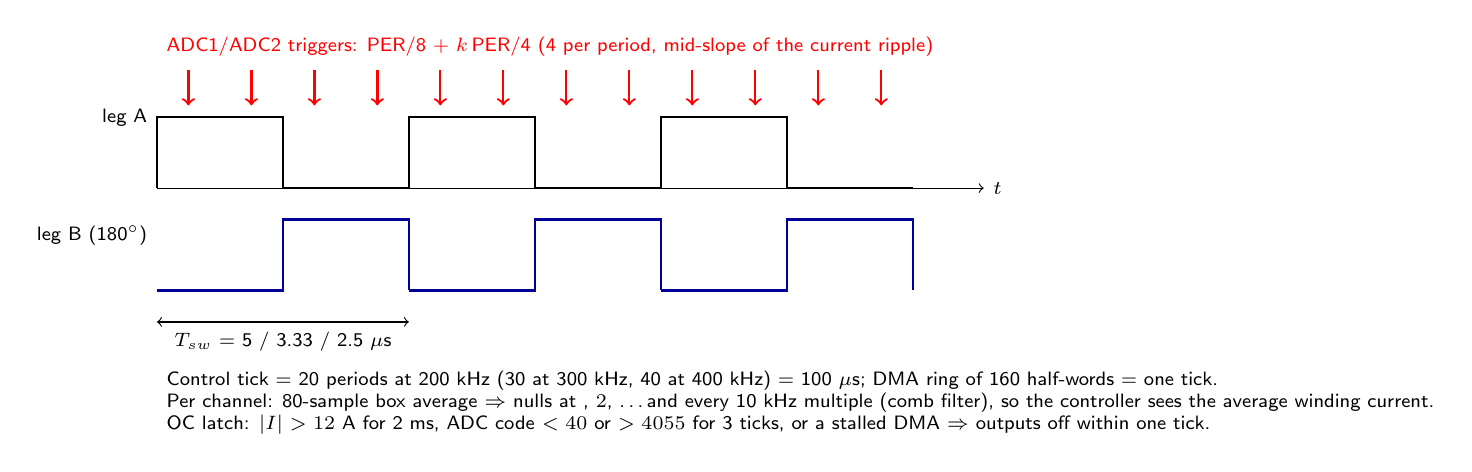
\begin{tikzpicture}[x=1cm,y=1cm,font=\sffamily\scriptsize]
  % PWM period axis
  \draw[->] (0,0) -- (10.5,0) node[right]{$t$};
  \foreach \i in {0,1,2}{
    \draw[thick] (\i*3.2,0) -- (\i*3.2,0.9) -- (\i*3.2+1.6,0.9) -- (\i*3.2+1.6,0) -- (\i*3.2+3.2,0);
  }
  \node[left] at (0,0.9) {leg A};
  \foreach \i in {0,1,2}{
    \draw[thick,blue!60!black] (\i*3.2,-1.3) -- (\i*3.2+1.6,-1.3) -- (\i*3.2+1.6,-0.4) -- (\i*3.2+3.2,-0.4) -- (\i*3.2+3.2,-1.3);
  }
  \node[left] at (0,-0.6) {leg B (180$^\circ$)};
  % triggers at PER/8 + k PER/4
  \foreach \i in {0,1,2}{\foreach \k in {0,1,2,3}{
    \draw[red,thick,->] (\i*3.2+0.4+\k*0.8,1.5) -- (\i*3.2+0.4+\k*0.8,1.05);
  }}
  \node[red,anchor=south west] at (0,1.55) {ADC1/ADC2 triggers: PER/8 + $k$\,PER/4 (4 per period, mid-slope of the current ripple)};
  \draw[<->] (0,-1.7) -- node[below]{$T_{sw}$ = 5 / 3.33 / 2.5 $\mu$s} (3.2,-1.7);
  \node[align=left,anchor=north west] at (0,-2.2) {Control tick = 20 periods at 200 kHz (30 at 300 kHz, 40 at 400 kHz) = 100 $\mu$s; DMA ring of 160 half-words = one tick.\\
  Per channel: 80-sample box average $\Rightarrow$ nulls at $\fsw$, $2\fsw$, \ldots and every 10 kHz multiple (comb filter), so the controller sees the average winding current.\\
  OC latch: $|I| > 12$ A for 2 ms, ADC code $<40$ or $>4055$ for 3 ticks, or a stalled DMA $\Rightarrow$ outputs off within one tick.};
\end{tikzpicture}
}
  \caption[{Hall-current sampling scheme}]{Hall-current sampling scheme: four HRTIM-triggered ADC conversions per switching period, box-averaged over one control tick.}
  \label{fig:adc}
\end{figure}

\subsection{Peripherals}
\begin{table}[htbp]\centering\scriptsize
\caption{Peripheral configuration (\code{shuffler\_hw.c/h}, \code{sensors.c}, \code{ina2x9.c}, \code{comms.c}).}
\label{tab:periph_full}
\begin{tabular}{l p{12.2cm}}
\toprule
HRTIM1 & $f_{HRTIM} = 170\,\mathrm{MHz}\times32 = 5.44$\,GHz (184\,ps). Master PER 27200 (200\,kHz) / 18133 (300) / 13600 (400). Legs A--D: A legs reset on master PER, B legs on master CMP2 = PER/2 (180$^\circ$ interleave). Duty = leg CMP1, preloaded, update on reset. Output 1 set on the master event, reset on CMP1; output 2 is the complement from the dead-time generator. Dead time \code{HW\_DEADTIME\_NS} 100 (136 steps $\times$ 0.735\,ns, both edges; was 200\,ns until 16 Oct). Pins: leg 0 S1A PA8/PA9, leg 1 S1B PA10/PA11, leg 2 S2A PB12/PB13, leg 3 S2B PB14/PB15 (AF13); a constructor drives them low before \code{main()}. Duty limits 0.05--0.95 (200\,kHz), 0.08--0.95 (300), 0.12--0.88 (400). Synchronised enable at master CMP1 = PER/4. Hardware fault inputs not used (COMP/DAC OC trip reserved, bit 0x002).\\
ADC1 / ADC2 & 12-bit, regular group of 2 ranks, trigger HRTIM ADC trigger 1 = TA CMP3/CMP4 + TB CMP3/CMP4 (4 per period at PER/8 + $k$PER/4). Sample time 6.5 cycles, clock PCLK/4 = 42.5\,MHz, no oversampling, offset calibration at start. ADC1 IN1 = PA0 ($I_{LA1}$), IN2 = PA1 ($I_{LA2}$); ADC2 IN17 = PA4 ($I_{LB1}$), IN7 = PC1 ($I_{LB2}$). DMA1 ch1/ch2 circular half-word, 160 samples = 4 triggers $\times$ 20 periods $\times$ 2 ranks = one control tick; the ISR polls the TC flags.\\
Hall conversion & $I = (\overline{\mathrm{code}} - \mathrm{zero})\cdot(3300/4096\,\mathrm{mV})/S$, $S = 100$\,mV/A on all four channels (B phases were 25 before 16 Oct; \code{params.yaml} still carries 25 for channels 1/3); nominal zero 2048 (1.65\,V); boot zero-cal averages 64 ticks, falls back to 2048 and sets \code{FLT\_ZEROCAL} if off by $>\pm124$ codes. B-phase sensors are physically reversed. Run-time \code{hall\_mva0..3} ($\pm$400, $|x|\ge10$), \code{hall\_zero0..3} (1800--2300). Box average of 80 samples per channel per tick (nulls at $\fsw$, $2\fsw$, \ldots and every 10\,kHz multiple). OC latch: $|I| > $ \code{oc\_a} (12\,A) for 20 ticks, code $<40$ or $>4055$ for 3 ticks, or DMA not wrapping for 3 ticks.\\
SPI3 & Master, mode 1, 8-bit MSB-first, software NSS, prescaler 128 $\Rightarrow$ 1.33\,MHz; PB3 SCK, PB4 MISO, PB5 MOSI; CS1 PA7 (U12, PV3+ to GND), CS2 PB6 (U11, PV2+ to GND), CS3 PC7 (U10 behind ISO7762 U13, PV1+ to PV3+). INA239 ADC\_CONFIG 0xF248 (continuous, 84\,$\mu$s, AVG 1); VBUS 3.125\,mV/LSB, die temperature 125\,m$^\circ$C/LSB; INA229 auto-detected (195.3\,$\mu$V/LSB); absent devices re-probed at 1\,Hz. $V_{M3} = U12$, $V_{M2} = U11 - U12$, $V_{M1} = -U10 - V_{M2}$ (U10 wired reversed) or, by default (\code{vm1\_src} = 2), $V_{M1} = v_{str,pi} - U11$ (stale after 2\,s).\\
LPUART1 & ST-LINK VCP PA2/PA3, 921600 8N1, blocking TX, protocol version 2, firmware \code{shuffler-fw-0.4.1}.\\
GPIO & E-stop PC0 (pull-up, falling-edge EXTI, prio 0); B1 toggles enable; LD2 PA5.\\
Controller filter & IIR $y_f \mathrel{+}= a(y - y_f)$, $a = 0.5569$ at $f_c = 2$\,kHz; optional moving average of 1--8 ticks (\code{filt\_ma}). Supervisor filter $\alpha = 0.2$.\\
\bottomrule
\end{tabular}
\end{table}

\subsection{Fault bits}
\begin{table}[htbp]\centering\small
\caption[{Firmware fault bitmask}]{Fault bitmask (\code{app.h}); OV/UV/string-OV need 3 consecutive 10\,ms samples; $V_{M1}$ is excluded unless \code{vm1\_prot} = 1.}
\label{tab:faults}
\begin{tabular}{l p{5.2cm} l p{5.2cm}}
\toprule
Bit & Meaning & Bit & Meaning\\
\midrule
0x001 & OC latch / ADC rail / DMA stall & 0x080 & over-temperature (INA die $>85\,^\circ$C)\\
0x002 & hardware OC (COMP, not implemented) & 0x100 & watchdog reset\\
0x004 & E-stop & 0x200 & software E-stop (\code{C,ESTOP})\\
0x008 & module OV $>30\V$ & 0x400 & string OV $>85\V$\\
0x010 & module UV $<3\V$ (closed loop only) & 0x800 & comms watchdog (CL, 5\,s without a command)\\
0x020 & zero-calibration & 0x1000 & $v_{str,pi}$ stale\\
0x040 & INA bus / VM unreadable & 0x2000 & main loop stalled $>20\ms$ while switching\\
\bottomrule
\end{tabular}
\end{table}

\subsection{Telemetry and command contract}
Telemetry frame (50\,Hz, 27 fields):
\begin{lstlisting}[language={},numbers=none]
T,ms,state,fault(hex),VM1,VM2,VM3,ILA1,ILB1,ILA2,ILB2,dA1,dB1,dA2,dB2,rv1,rv2,beta,stress,IM1r,IM2r,T1,T2,T3,kscale,pset,pver
S,ms,state,fault,mode,fw,pver        F,ms,code,channel,value,raw        A,<cmd>,OK|ERR,<why>        P,name,val[,min,max,class]
\end{lstlisting}
States: \code{BOOT, SELFTEST, IDLE, SOFTSTART, RUN\_OL, RUN\_CL, RUN\_OL1, RUN\_CL1, RUN\_OL2, RUN\_CL2, STOP, FAULT}. Outside RUN\_CL the fields \code{rv}, \code{beta}, \code{stress}, \code{IM1r}, \code{IM2r} repeat their last value (the ``stale values'' seen on the Grafana screenshots); the analysis keeps RUN rows only.

Commands (Pi $\rightarrow$ Nucleo): \code{C,MODE,<IDLE|OL|CL|OL1|CL1|OL2|CL2>}; \code{C,TEST,0..3}; \code{C,EN,0|1}; \code{C,DUTY,leg,d}; \code{C,DUTYS,dA1,dB1,dA2,dB2}; \code{C,VREF,rv1,rv2}; \code{C,SUP,0|1}; \code{C,SET,name,value}; \code{C,SETM,m00..m33}; \code{C,GET,name}; \code{C,LIST}; \code{C,APPLY}; \code{C,REVERT}; \code{C,CAL,ch,mV/A,zero}; \code{C,ESTOP}; \code{C,CLEAR}; \code{C,PING}. Parameter classes: STAGED (take effect on \code{C,APPLY}: \code{kscale}, \code{kp\_v}, \code{kp\_i}, \code{fc\_lpf}, \code{filt\_ma}, \code{dmin}, \code{dmax}, \code{m00..m33}); LIVE (\code{sup\_*}, \code{vref1/2}, \code{hall\_mva*}, \code{oc\_a}, \code{vm\_ov}, \code{vm\_uv}, \code{vstr\_ov}, \code{vstr\_param}, \code{vstr\_pi}, \code{vm1\_prot}, \code{slew}, \code{wdg\_s}); IDLE-only (\code{hall\_zero*}, \code{vm1\_src}). \code{pset} increments on every swap; a swap rebases the integrators ($\xi = M^{-1} u_{act}$) so the duties do not jump.

\subsection{Firmware images}
\begin{table}[htbp]\centering\small
\caption{Firmware variants used on 16 and 20 Oct (\code{7\_Pi/firmware/VERSION.txt}).}\scriptsize
\label{tab:fwimages}
\begin{tabular}{l r r r l l}
\toprule
Image & $\fsw$ [kHz] & PER & periods / tick & duty limits & gain set (\code{pver})\\
\midrule
\code{shuffler.bin} & 200 & 27200 & 20 & 0.05--0.95 & \code{20261015-1950-3mod-qspice200-bench}\\
\code{shuffler\_300k.bin} & 300 & 18133 & 30 & 0.08--0.95 & \code{20261016-1628-3mod-qspice300-bench}\\
\code{shuffler\_400k.bin} & 400 & 13600 & 40 & 0.12--0.88 & \code{20261016-1751-3mod-qspice400-bench}\\
\bottomrule
\end{tabular}
\end{table}

\subsection{Raspberry Pi stack}
{\sloppy Docker: \code{influxdb:2.7} on :8086 (org \code{boost}, bucket \code{shuffler}, infinite retention) and \code{grafana/grafana-oss:11.2.0} on :3000 (provisioned Flux datasource, dashboard ``Shuffler pod'': mode, active, init check, temperatures, state, module voltages, inductor currents, duties, supervisor, reconstructed module currents, string voltage INA-sum vs e-load, e-load status/V/I, string power, command log, run-time parameters). Services (systemd): \code{pod.service} (\code{pod.py}, 921600 baud), \code{eload.service} (Rigol DL3021 over USB-TMC, 5\,Hz measurements, 2\,Hz $V_{str}$ forward, limits CC 15\,A / CV 150\,V / CP 200\,W), \code{params\_web.service} (stdlib HTTP on :8080, no authentication, allow-listed commands). IR: Elegoo NEC remote via \code{gpio-ir} on GPIO17 (POWER = E-stop, FUNC = disable, digits = presets, PLAY = run, VOL$\pm$ = kscale $\pm0.1$, EQ = status pages). Presets (\code{actions.py}): 0 init check, 1 open loop, 2 closed loop, 3/4 load on/off, 5/6 load remote/local, 7/8 kscale 0.3/1.0, 9 clear fault. Flashing: OpenOCD (\code{interface/stlink.cfg}, \code{target/stm32g4x.cfg}) with the pod stopped around the flash; \code{stage\_firmware.sh} builds Release and copies the \code{.bin}; \code{sync.sh} rsyncs \code{7\_Pi} to the Pi; \code{setup.sh} installs packages, udev rules, overlays (I$^2$C LCD 0x27/0x3F, 1-wire DS18B20 GPIO4, IR GPIO17), the venv and the services.\par}

\note{Inconsistencies found while documenting (fix in the repository or mention): the README says IWDG 2\,s and dead time 200\,ns where the code says 0.3\,s and 100\,ns; \code{telemetry.md} says \code{\%.4g} where the code prints fixed decimals; \code{params.yaml} still has 25\,mV/A for the B-phase halls; no script builds the 300\,kHz and 400\,kHz images; and there is no MISRA statement although the proposal promised MISRA-C.}
